\chapter{CodeSmith}
\label{cha:codeSmith}


%----------
\section{Template Syntax}
CodeSmith \cite{CodeSmith} is a freeware template-based code generator which is able to 
generate code for any ASCII-based language. The syntax for creating 
CodeSmith templates is close to the ASP.NET syntax.

A template source file consists of template code and the static part of the 
desired source code output. In Listing \ref{lst:simpleExample} you can see 
an example. Everything encapsulated in \verb~<% %>~ tags will be 
replaced by CodeSmith, the rest be printed as is.

There are varieties of this tags. \verb~<%@~ is the beginning of a 
compiler directive. On the line 1 of Listing \ref{lst:simpleExample} you 
can see the \verb~CodeTemplate~ directive. This is the first and only 
mandatory code block in a template. It needs a \verb~Language~ attribute 
specifying the template language and a \verb~TargetLanguage~ attribute 
defining the language of generated code output. A \verb~Description~ 
attribute can be given optionally.

The \verb~Property~ directive you see at line 3 declares a property 
with a \verb~Name~ and a \verb~Type~ as mandatory attributes. This is exactly 
the same as a .NET property. The attribute \verb~Category~ defines
the Section where the property is shown in the GUI. The given category on 
line 3 of Listing \ref{lst:simpleExample} can be found in the section title 
of the \verb~ClassName~ property in Figure \ref{fig:codesmithGUI}. If no 
category is specified the property will be shown in the misc section.

\begin{lstlisting}[float,caption=Simple Example,label=lst:simpleExample]
<%@ CodeTemplate Language="C#" TargetLanguage="C#"
                 Description="This is a sample template." %>
<%@ Property Name="ClassName" Type="System.String" Category="Design"
             Default="MyClass1" Description="Name of class to create" %>

public class <%= ClassName %>() {

   <%= ClassName %>() {
   }
}
\end{lstlisting}

A code block beginning with \verb~<%=~ contains only one property like at 
lines 6 and 8 in Listing \ref{lst:simpleExample}. It is a short form to 
print that property. You can see the result of the template code in Listing 
\ref{lst:simpleExample} in Figure \ref{fig:codesmithGUI}.

\begin{figure}[H]
	\begin{center}
		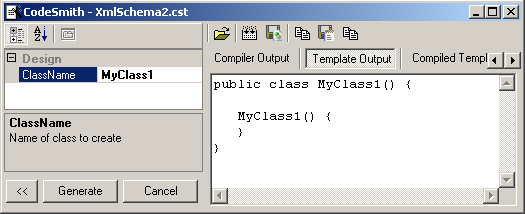
\includegraphics[width=9cm]{./files/inc/figures/codesmithGUI}
		\caption{\label{fig:codesmithGUI}CodeSmith GUI}
	\end{center}
\end{figure}


%-----
\subsection{Functions}
Template code can contain any logic like a loop for iterating, an 
\verb~if~ clause or anything else. If code is too complex to manage 
in a template there is the possibility to write functions. Usually 
they are placed at the end of a template in a \verb~<script>~ section 
as shown in Listing \ref{lst:script}.

\begin{lstlisting}[float,caption=$<$script$>$ section,label=lst:script]
<script runat="template">
public string getEmail(string forename, string name)
{
	string email = forename + "." + name + "@hsr.ch";
	return email;
}
</script>\end{lstlisting}


%-----
\subsection{Derive from ``code behind''}
For more complex templates it could be useful to split the code into two 
files. The template file will only consists of static text and as few logic 
as possible. Only some simple loops or decisions. The main logic can be 
packed into a class placed in an external file. Such code is called ``code 
behind'' because you don't see it while working on the template.

This class has to be derived from the \verb~CodeTemplate~ class in the namespace 
\verb~CodeSmith.Engine~ as shown in Listing \ref{lst:codebehind} at line 1 and 5. The 
code template has to inherit from this class. How to reference the external 
file in the template and inherit from the class in it is shown in Listing 
\ref{lst:derive}.

\begin{lstlisting}[caption=Code behind (sample1.cst.cs),label=lst:codebehind]
using CodeSmith.Engine;

namespace SampleNamespace
{
	public class Sample1 : CodeTemplate
	{
		private string className;
		
		public Sample1() { }
		
		public string ClassName {
			get{ return value; }
			set{ className = value; }
		}
	}
}
\end{lstlisting}

\begin{lstlisting}[caption=Include a base class (sample1.cst),label=lst:derive]
<%@ CodeTemplate Src="sample1.cst.cs" Inherits="SampleNamespace.Sample1"
                 Language="C#" TargetLanguage="C#" %>
                 
public class <%= ClassName %>() {

   <%= ClassName %>() {
   }
}
\end{lstlisting}

Properties in a class you derive from must implement \verb~set~ and \verb~get~ 
methods because CodeSmith treats such a property like those declared with 
directives. CodeSmith has to read them to show the values in the GUI. And it 
has to manipulate them if you change a value over the GUI or generate code 
with an external configuration as described later.

All the properties and methods in such a class can be accessed directly from 
inline code as you see in Listing \ref{lst:derive} at line 4 and 6.


%-----
\subsection{Logic in an assembly}
Another possibility to separating the logic from template code is to use an 
assembly. Listing \ref{lst:assemblyTpl} shows the usage of an assembly. 
There are two directives needed. The directive at line 3 specifies an assembly 
without the .dll extension. It needs to be in either the same directory as the 
template or in the same directory as the CodeSmith executable.

Now you can make instances of each class in that assembly. The line 2 in Listing 
\ref{lst:assemblyTpl} shows how to make an instance of the class \verb~Sample2~ 
in the namespace \verb~SampleNamespace~. The property \verb~FileObject~ represents 
the instance. You can access all properties and methods of this object like shown 
in line 7 of Listing \ref{lst:assemblyTpl}

\begin{lstlisting}[float,caption=Use an Assembly,label=lst:assemblyTpl]
<%@ CodeTemplate Language="C#" TargetLanguage="C#" %>
<%@ Property Name="FileObject" Type="SampleNamespace.Sample2" %>
<%@ Assembly Name="ASample" %>

public SampleClass {
  public static void main() {
    Console.WriteLine("Selected file: {0}", <%= FileObject.File %>);
  }
}
\end{lstlisting}

The property defined in the template in that case is an object. This object can have 
several properties. That is why it is needed to implement an \verb~Editor~, which enables 
you to set the properties of that object with the CodeSmith GUI. Such an \verb~Editor~ is a 
.NET technologie to edit the properties of an object which is bound to a input field 
in a GUI. If you bind your own object to an input field you have to write your own 
\verb~Editor~.

For this the assembly must provide a form for a modal dialog or a drop-down box 
which is designed to set all the properties. To show the settings in the GUI, 
CodeSmith calls the \verb~ToString()~ method. To have any effect on the text showed 
in the GUI you can overwrite the \verb~ToString()~ method.

Listings \ref{lst:assemblyClass} and \ref{lst:assemblyClassEditor} use a 
default \verb~OpenFileDialog~ to demonstrate this functionality. Line 6 and 7 
of Listing \ref{lst:assemblyClass} is defined which \verb~Editor~ to use. Listing 
\ref{lst:assemblyClassEditor} shows the implementation of such an \verb~Editor~.

\begin{lstlisting}[caption=Assembly source,label=lst:assemblyClass]
using System;
using System.ComponentModel;

namespace SampleNamespace
{
	[Editor(typeof(SampleNamespace.Sample2Editor),
	        typeof(System.Drawing.Design.UITypeEditor))]
	public class Sample2 
	{
		private string m_file = "";

		public Sample2()
		{
		}

		public string File 
		{ 
			get { return m_file; } 
			set { m_file = value; } 
		}
	
		public override string ToString() {	return m_file; }
	}
}
\end{lstlisting}

\begin{lstlisting}[caption=Editor,label=lst:assemblyClassEditor]
using System;
using System.ComponentModel;
using System.Windows.Forms;
using System.Drawing.Design;

namespace SampleNamespace
{
	public class Sample2Editor : UITypeEditor
	{
		public Sample2Editor() : base() {}

		public override object EditValue(ITypeDescriptorContext context,
		                                 IServiceProvider provider,
		                                 object obj) 
		{
			if (provider != null)
			{
				OpenFileDialog fileDialog = new OpenFileDialog();

				if(fileDialog.ShowDialog() == DialogResult.OK)
				{
					obj = new Sample2();
					((Sample2)obj).File = fileDialog.FileName;
				}
			}
			return obj;
		}

		public override
		UITypeEditorEditStyle GetEditStyle(ITypeDescriptorContext context) 
		{
			return UITypeEditorEditStyle.Modal;
		}
	}
}
\end{lstlisting}

If you click into the input field in the CodeSmith GUI the method 
\verb~EditValue()~ will be called. This opens the \verb~FileOpenDialog~ 
and sets the property \verb~File~ after closing the dialog.

The method \verb~GetEditStyle()~ tells the CodeSmith GUI what kind of input 
box to provide. Either a drop-down box or a modal dialog are possible. For 
the \verb~FileOpenDialog~ you have to set \verb~Modal~ (see Listing 
\ref{lst:assemblyClassEditor},line 32). This results in a button with three 
dots like you can see next to the input box of \verb~FileObject~ in Figure 
\ref{fig:codesmithGUI2}.

\begin{figure}[thb]
	\begin{center}
		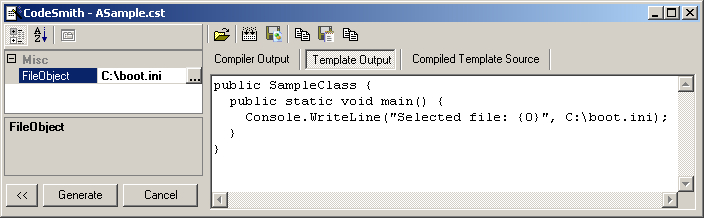
\includegraphics[width=12cm]{./files/inc/figures/codesmithGUI2}
		\caption{\label{fig:codesmithGUI2}Input box for an assembly}
	\end{center}
\end{figure}


%----------
\section{Code generation}
\label{sec:codeSmithGeneration}

If you want to generate code for several values it is a drawback that you have 
to set all the properties by hand. That's why you can can use an external file 
as input for the generation process. This procedure is described in the 
following section.


%-----
\subsection{XML configuration file}
There are two ways to generate code without the CodeSmith GUI. You can choose between 
a command line tool and the possibility to 
integrate the generation into Microsoft Visual Studio .NET. Both take 
the settings from an xml file like in Listing \ref{lst:xmlConfig}. 

The specified \verb~namespace~ at line 3 is optional and encloses the whole 
generated code from all defined \verb~propertySet~s.
The \verb~imports~ given at lines 5 and 6 are included at the top of the generated 
code with the \verb~using~ keyword.
For each \verb~propertySet~ defined in the \verb~propertySets~ element CodeSmith 
generates code with the properties specified in it.

\begin{lstlisting}[float,language=XML,caption=xml configuration,label=lst:xmlConfig]
<?xml version="1.0" encoding="utf-8" ?>
<codeSmith>
	<namespace>MyNamespace</namespace>
	<imports>
		<import namespace="System" />
		<import namespace="System.Collections" />
	</imports>
	<propertySets>
		<propertySet>
			<property name="FileName">BusinessObj1.dll</property>
		</propertySet>
		<propertySet>
			<property name="FileName">BusinessObj2.dll</property>
		</propertySet>
	</propertySets>
	<template path="BusinessObjects.cst" />
</codeSmith>
\end{lstlisting}

\noindent The command line to generate code is:\\
\indent \verb~CodeSmithConsole.exe sample1.xml output.cs~

\noindent The first filename specifies the xml configuration file. The second filename 
is optional. If specified, the generated code is written to that file, otherwise 
the output is shown on stdout. 

%-----
\subsection{Visual Studio .NET integration}
To run the generation of code from within the Visual Studio you have to add the xml 
configuration file to the Visual Studio project. Then you have to set the 
property \verb~Custom Tool~ to \verb~CodeSmithGenerator~ as shown in Figure 
\ref{fig:codesmithVsdotnet} on the right.

The \verb~Build Action~ field has to be set to \verb~Content~. This causes Visual Studio 
to execute the generation every time the content of the xml file has changed. The generation 
of the code can also be initiated by right clicking the xml file and select 
\verb~Run Custom Tool~.

\begin{figure}[thb]
	\begin{center}
		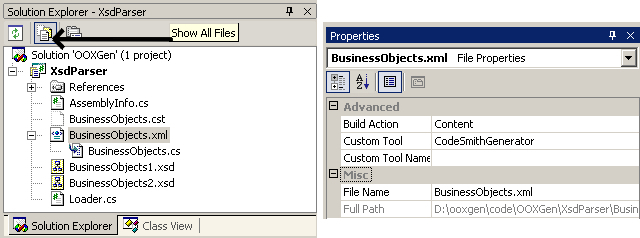
\includegraphics[width=11cm]{./files/inc/figures/codesmithVsdotnet}
		\caption{\label{fig:codesmithVsdotnet}Visual Studio .NET integration}
	\end{center}
\end{figure}

If the option \emph{Show All Files} (see Figure \ref{fig:codesmithVsdotnet}) is 
turned on, the generated file is displayed as a child of the xml file.